\chapter{SYSTEM ANALYSIS }
 
 \section{Module Description}
 The "Shopify" platform is divided into multiple functional modules, each playing a key role in ensuring smooth operation, seamless shopping, and an engaging user experience. The main modules include:
 \begin{itemize}
    \item \textbf{User Authentication Module:} This module is responsible for handling how users (both buyers and sellers) register and log into the system. It processes user credentials securely and manages session states, ensuring that personalized data is accessible only to authenticated individuals.
    \item \textbf{Seller Dashboard Module:} The application provides a dedicated dashboard for sellers. This module enables sellers to manage their store, add new products, update inventory, and analyze their performance. It ensures that product modifications are accurately reflected across the platform.
    \item \textbf{Product Catalog \& Search Module:} This module manages the display of products to buyers. It includes advanced search functionalities and semantic product embeddings that allow the system to recommend conceptually similar products to the user based on their browsing behavior.
    \item \textbf{Order Management Module:} This module tracks the transaction state and fulfillment progress of orders. It utilizes tracking IDs to provide buyers with real-time updates on their purchases and allows sellers to manage incoming requests.
    \item \textbf{UI \& Interaction Module:} The user interface plays a major role in the shopping experience. Built using React and Tailwind CSS, this module ensures that the interface is clear, responsive, and easy to navigate across all devices.
\end{itemize}

\section{Business Rules}
Business rules are specific guidelines, conditions, or constraints that govern the operations of a business or system. They define how processes and activities should be conducted to ensure consistency, fairness, and alignment with business objectives.\\\\
\textbf{Product Management}
\begin{itemize}
    \item Only authenticated users with a "Seller" role can add or modify products within the system.
    \item Products must contain accurate descriptions, pricing, and category information before they can be published.
    \item The system processes product descriptions to generate embedding vectors for refined similarity searches.
\end{itemize}
\textbf{Order Processing}
\begin{itemize}
    \item An order can only be confirmed once a valid payment method has been verified.
    \item A unique tracking ID is generated for every confirmed order to allow buyers to track fulfillment status.
    \item Sellers must update the order status promptly to keep buyers informed.
\end{itemize}

\newpage
\section{Analysis of Architecture}
{\large \textbf{Laravel \& React Ecosystem}}\\\\
Shopify utilizes Laravel for robust backend operations and data management, and React for a dynamic, highly responsive frontend experience. The integration is smoothed out using Inertia.js, allowing the platform to behave as a Single Page Application (SPA) without the traditional API overhead.\\\\
\begin{enumerate}
    \item \textbf{Backend Foundation (Laravel):}
    \begin{itemize}
        \item Provides secure routing, authentication, and session management.
        \item Utilizes Eloquent ORM for streamlined interaction with the relational database.
    \end{itemize}
    \item \textbf{Frontend Dynamism (React):}
    \begin{itemize}
        \item Handles complex state management for shopping carts and user interfaces.
        \item Employs responsive design principles using Tailwind CSS.
    \end{itemize}
    \item \textbf{Data Flow (Inertia.js):}
    \begin{itemize}
        \item Removes the need to build separate REST APIs for the frontend.
        \item Passes data directly from Laravel controllers to React components as props.
    \end{itemize}
\end{enumerate}

\section{Project Pipeline}
\begin{figure}[H]
    \centering
    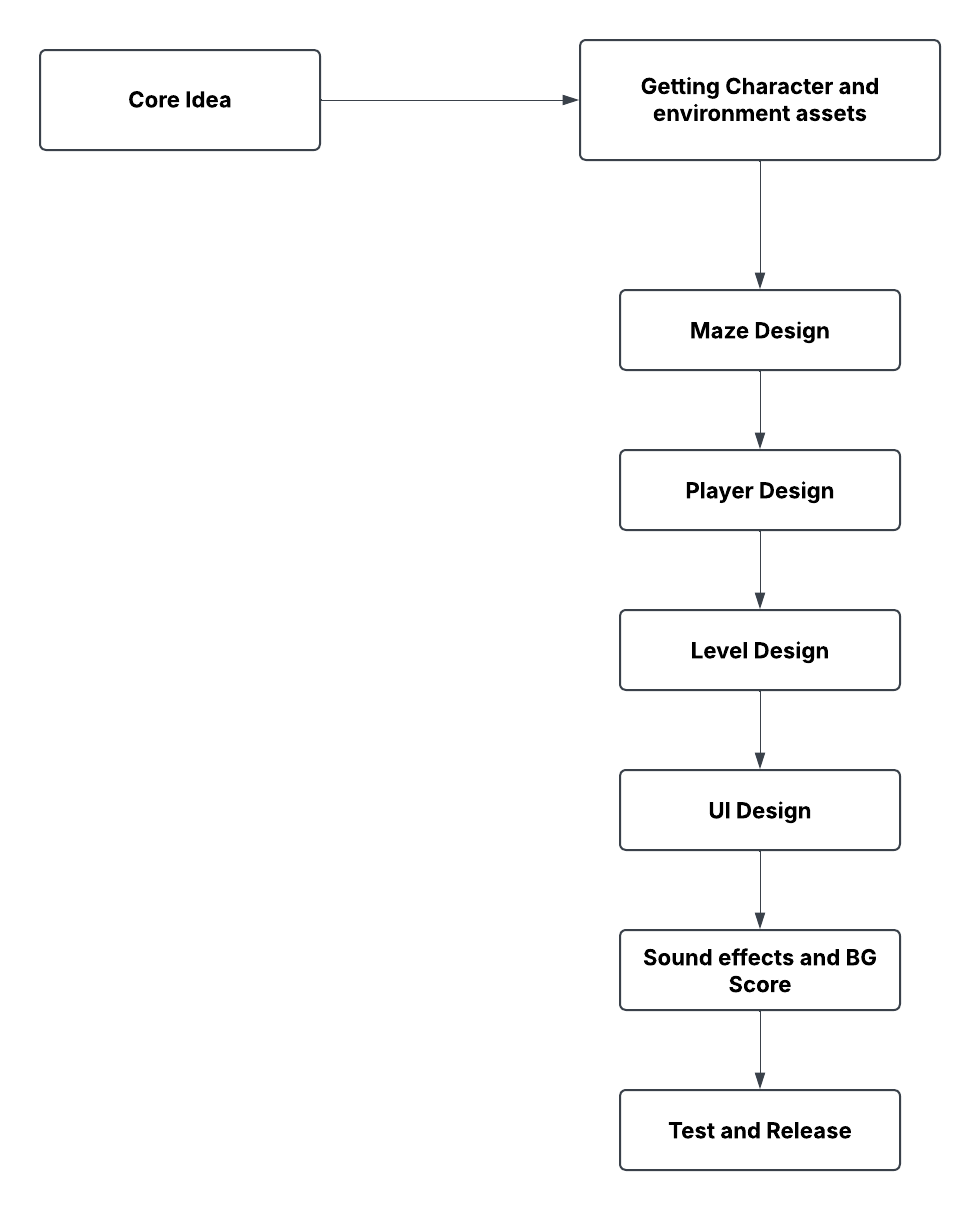
\includegraphics[width=0.8\textwidth]{project_pipe.png}
    \caption{Project Pipeline}
    \label{fig:project_pipeline}
\end{figure}

 \section{Feasibility Analysis}
 
 \subsection{Technical Feasibility}
 Technical feasibility assesses whether a project can be successfully developed and implemented using the current available technology, skills, and resources.\\\\
 \noindent
The technologies chosen for the Shopify project are highly feasible and industry-standard. The frontend utilizes React to provide an interactive interface, while Tailwind CSS ensures rapid, consistent styling. The backend is powered by Laravel, a proven PHP framework that simplifies complex tasks like routing, sessions, and caching. The integration of Inertia.js bridges these technologies seamlessly. Code, databases, and assets are managed using established tools, ensuring a scalable and efficient platform.

 \subsection{Economical Feasibility}
 Economic feasibility refers to the assessment of the financial aspects of a project to determine whether it is cost-effective and viable.\\\\
 The economic feasibility of Shopify is high. Development costs are minimized by utilizing free and open-source frameworks (Laravel, React, Tailwind CSS). The infrastructure required can start small, utilizing basic cloud hosting for PHP/MySQL, and can easily scale as the platform grows. Ongoing maintenance costs are predictable and manageable, making it an economically sound project.
 
 \subsection{Operational Feasibility}
 Operational feasibility evaluates whether the project aligns with operational requirements and whether it can be smoothly integrated into existing processes.\\\\
 The operational feasibility of Shopify evaluates how effectively the system can handle user registrations, product listings, and order processing. The intuitive interface ensures that both buyers and sellers can navigate the platform with minimal training. Features like the seller dashboard and automated product embeddings significantly improve the operational efficiency of managing an e-commerce platform. The system is highly adaptable and user-friendly, confirming strong operational feasibility.

 \section{System Environment}
 
 \subsection{Software Environment}
 \textbf{Backend Framework:} Laravel (PHP 8+)\\\\
 \textbf{Frontend Library:} React.js\\\\
 \textbf{Integration Layer:} Inertia.js\\\\
 \textbf{Styling:} Tailwind CSS\\\\
 \textbf{Database:} MySQL / PostgreSQL (managed via Laravel Migrations)\\\\
 \textbf{Asset Bundler:} Vite
 
 \subsection{Hardware Environment}
 \textbf{Processor (CPU):} Any modern multi-core processor (e.g., i5 12th Gen or equivalent)\\\\
 \textbf{Memory (RAM):} 8 GB minimum (16 GB recommended for development)\\\\
 \textbf{Storage:} 256 GB SSD\\\\
 \textbf{Operating System:} Windows, macOS, or Linux
 \newpage
 
 \section{Actors and roles}
 The system involves two primary actors: Buyers and Sellers.\\\\
\noindent
\textbf{Actors name:} Buyer
\\\\
 \textbf{Role:}
 \begin{itemize}
    \item Browse products and categories.
    \item Add items to the cart and proceed to checkout.
    \item Track order status using tracking IDs.
    \item Manage personal profile and shipping details.
\end{itemize}
\noindent
\textbf{Actors Name:} Seller
\\\\
\textbf{Role:}
\begin{itemize}
    \item Manage product inventory (add, edit, delete products).
    \item Monitor incoming orders and update fulfillment status.
    \item View store analytics and performance metrics via the Seller Dashboard.
\end{itemize}
